\section{Deep Learning}
\label{sec:deep-learning}

A neural network is a function that learns the relationship between its
inputs and outputs from data. It adjusts internal values each time it
processes an example, gradually producing more accurate outputs. The
network is built from many copies of one simple unit, and the way these
units are arranged determines what the network can learn.

\subsection{Neurons}
\label{subsec:neurons}

A \emph{neuron} takes several numbers as input, combines them, and
produces a single number as output. Each input is scaled by its own
number, and these numbers control how much each input matters.

\smallskip
These numbers are called \emph{weights}. A large weight means that
input matters more, and a weight near zero means it is mostly ignored.
The neuron learns which combinations of inputs are relevant by
adjusting these weights.

\smallskip
Each input is multiplied by its weight, a \emph{bias} term is added,
and the result is passed through an \emph{activation function}:
%
\begin{align}
\label{eq:neuron-z}
z &= w_1 x_1 + w_2 x_2 + w_3 x_3 + b \\
\label{eq:neuron-a}
a &= \sigma(z)
\end{align}
%
where $x_1, x_2, x_3$ are the inputs, $w_1, w_2, w_3$ are the
weights, $b$ is the bias, $\sigma$ is the activation function, $z$ is the
weighted sum, and $a$ is the neuron's output. The bias shifts the output
independently of the inputs, allowing the neuron to produce a nonzero
result even when all inputs are zero.

\smallskip
This output is the neuron's prediction for the given inputs. The weights
and bias are the neuron's \emph{parameters}, the values that change
during training.

\begin{figure}[ht]
\centering
% Thesis-wide categorical color palette
% Usage: % Thesis-wide categorical color palette
% Usage: \input{figures/palette} in any figure file
%
% Muted primary colors -- print-friendly, visually distinct.
% Inspired by Cooper Union's red/blue primaries, softened for
% academic figures. Use palA-palC for data series in scatter
% plots, line charts, bar charts, etc.

\definecolor{palA}{HTML}{1F77B4}   % Tableau blue
\definecolor{palB}{HTML}{D62728}   % Tableau red
\definecolor{palC}{HTML}{2CA02C}   % Tableau green
 in any figure file
%
% Muted primary colors -- print-friendly, visually distinct.
% Inspired by Cooper Union's red/blue primaries, softened for
% academic figures. Use palA-palC for data series in scatter
% plots, line charts, bar charts, etc.

\definecolor{palA}{HTML}{1F77B4}   % Tableau blue
\definecolor{palB}{HTML}{D62728}   % Tableau red
\definecolor{palC}{HTML}{2CA02C}   % Tableau green

\definecolor{nodeblue}{HTML}{B8D2E6}
\definecolor{nodeborder}{HTML}{5A87B5}
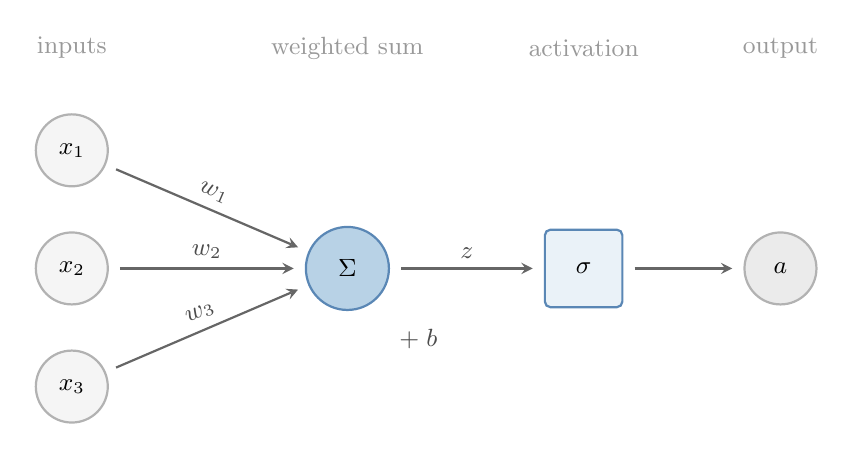
\begin{tikzpicture}[
    inputnode/.style={circle, draw=black!30, thick, fill=black!4,
                      minimum size=26pt, inner sep=0pt},
    sumnode/.style={circle, draw=nodeborder, thick, fill=nodeblue,
                    minimum size=30pt, inner sep=0pt},
    actnode/.style={rectangle, draw=nodeborder, thick, fill=nodeblue!30,
                    minimum width=28pt, minimum height=28pt,
                    inner sep=2pt, rounded corners=2pt},
    outputnode/.style={circle, draw=black!30, thick, fill=black!8,
                       minimum size=26pt, inner sep=0pt},
    conn/.style={->, thick, >=stealth, black!60},
    mathlbl/.style={font=\small, text=black!70},
    seclbl/.style={font=\small, text=black!40},
]

% --- Input nodes (math variable inside) ---
\node[inputnode] (x1) at (0, 1.5)  {\small $x_1$};
\node[inputnode] (x2) at (0, 0)    {\small $x_2$};
\node[inputnode] (x3) at (0, -1.5) {\small $x_3$};

% --- Summation node ---
\node[sumnode] (sum) at (3.5, 0) {\small $\Sigma$};

% --- Bias label (below-right of sum node) ---
\node[mathlbl] at (4.4, -0.9) {$+\; b$};

% --- Connections with weight labels ---
\draw[conn, shorten >=4pt, shorten <=4pt] (x1) -- (sum) node[mathlbl, midway, above, sloped] {$w_1$};
\draw[conn, shorten >=4pt, shorten <=4pt] (x2) -- (sum) node[mathlbl, midway, above, sloped] {$w_2$};
\draw[conn, shorten >=4pt, shorten <=4pt] (x3) -- (sum) node[mathlbl, midway, above, sloped] {$w_3$};

% --- Activation function ---
\node[actnode] (act) at (6.5, 0) {\small $\sigma$};
\draw[conn, shorten >=4pt, shorten <=4pt] (sum) -- (act) node[mathlbl, midway, above] {$z$};

% --- Output ---
\node[outputnode] (out) at (9.0, 0) {\small $a$};
\draw[conn, shorten >=4pt, shorten <=4pt] (act) -- (out);

% --- Section labels above ---
\node[seclbl] at (0, 2.8) {inputs};
\node[seclbl] at (3.5, 2.8) {weighted sum};
\node[seclbl] at (6.5, 2.8) {activation};
\node[seclbl] at (9.0, 2.8) {output};

\end{tikzpicture}
\caption{A single neuron. Each input is multiplied by a weight, the
  results are summed with a bias, and the total is passed through an
  activation function to produce the output.}
\label{fig:neuron}
\end{figure}


\begin{example}
\label{ex:neuron}
Suppose the three inputs have values $x_1 = 2.0$, $x_2 = -1.0$,
$x_3 = 0.5$, with weights $w_1 = 0.4$, $w_2 = 0.6$, $w_3 = -0.2$, and
bias $b = 0.1$. The weighted sum is:
%
\begin{align*}
z &= (0.4)(2.0) + (0.6)(-1.0) + (-0.2)(0.5) + 0.1 \\
  &= 0.8 - 0.6 - 0.1 + 0.1 \\
  &= 0.2
\end{align*}
%
Notice that $w_2 = 0.6$ is the largest weight, so $x_2$ contributes the
most to the sum. The weighted sum is $z = 0.2$. Applying the activation
function gives the neuron's output $a = \sigma(0.2)$.
\end{example}

\smallskip
The most widely used activation function is the \emph{rectified
linear unit} (ReLU), which passes positive values through and sets
negative values to zero:
%
\begin{align}
\label{eq:relu}
\text{ReLU}(x) &= \max(0,\, x) \\[4pt]
\notag
               &= \begin{cases}
                  0 & \text{if } x \leq 0 \\
                  x & \text{if } x > 0
                  \end{cases}
\end{align}
%
With $z = 0.2$, $\text{ReLU}(0.2) = 0.2$, so the neuron's output is
$a = 0.2$. If the weighted sum had been $-0.3$, the output would be
$a = 0$.%
\footnote{Earlier activation functions such as the sigmoid and
hyperbolic tangent (tanh) have been largely replaced by ReLU in
modern architectures.}

\smallskip
The weights and bias start with arbitrary values, so the neuron's first
predictions are wrong. Training adjusts the parameters once it can
measure how wrong each prediction is.

\begin{figure}[ht]
\centering
% Thesis-wide categorical color palette
% Usage: % Thesis-wide categorical color palette
% Usage: \input{figures/palette} in any figure file
%
% Muted primary colors -- print-friendly, visually distinct.
% Inspired by Cooper Union's red/blue primaries, softened for
% academic figures. Use palA-palC for data series in scatter
% plots, line charts, bar charts, etc.

\definecolor{palA}{HTML}{1F77B4}   % Tableau blue
\definecolor{palB}{HTML}{D62728}   % Tableau red
\definecolor{palC}{HTML}{2CA02C}   % Tableau green
 in any figure file
%
% Muted primary colors -- print-friendly, visually distinct.
% Inspired by Cooper Union's red/blue primaries, softened for
% academic figures. Use palA-palC for data series in scatter
% plots, line charts, bar charts, etc.

\definecolor{palA}{HTML}{1F77B4}   % Tableau blue
\definecolor{palB}{HTML}{D62728}   % Tableau red
\definecolor{palC}{HTML}{2CA02C}   % Tableau green

\definecolor{nodeblue}{HTML}{B8D2E6}
\definecolor{nodeborder}{HTML}{5A87B5}
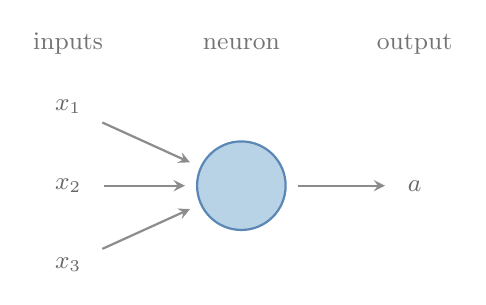
\begin{tikzpicture}[
    val/.style={font=\small, text=black!60, inner sep=2pt},
    neuron/.style={circle, draw=nodeborder, thick, fill=nodeblue,
                   minimum size=32pt, inner sep=0pt},
    conn/.style={->, thick, >=stealth, black!45},
]

% --- Input values ---
\node[val] (x1) at (-2.2, 1.0)  {$x_1$};
\node[val] (x2) at (-2.2, 0)    {$x_2$};
\node[val] (x3) at (-2.2, -1.0) {$x_3$};

% --- Neuron ---
\node[neuron] (n) at (0, 0) {};

% --- Input connections ---
\draw[conn, shorten >=4pt, shorten <=6pt] (x1) -- (n);
\draw[conn, shorten >=4pt, shorten <=6pt] (x2) -- (n);
\draw[conn, shorten >=4pt, shorten <=6pt] (x3) -- (n);

% --- Output value ---
\node[val] (out) at (2.2, 0) {$a$};
\draw[conn, shorten >=6pt, shorten <=4pt] (n) -- (out);

% --- Section labels ---
\node[val, text=black!55] at (-2.2, 1.8) {inputs};
\node[val, text=black!55] at (0, 1.8) {neuron};
\node[val, text=black!55] at (2.2, 1.8) {output};

\end{tikzpicture}
\caption{The same neuron drawn as a single unit. Each circle in
  a network diagram represents the full computation from
  \cref{fig:neuron}.}
\label{fig:neuron-abstract}
\end{figure}


\subsection{Loss Functions}
\label{subsec:loss-functions}

A neural network begins with random weights -- its outputs are
meaningless. Training is the process of adjusting those weights so
that the network's outputs match the desired outputs. This is an
optimization problem: find a setting of the weights that minimizes
some measure of how wrong the network is.

\smallskip
That measure is called the \emph{loss function}. Different tasks
call for different loss functions, but the training procedure is
the same regardless of which loss is used. The loss is a single
number that summarizes how far the network's predictions are from
the correct answers; training drives this number down.

\smallskip
For tasks where the network predicts a continuous value -- such as
estimating a Q-value -- the standard loss is the \emph{mean squared
error} (MSE): the average squared difference between the predicted
and target values. Squaring means that large errors are penalized
more heavily than small ones, so MSE prioritizes correcting the
worst predictions first. This is the loss that appears in the
function approximation setting of \cref{eq:fa-loss}.

\smallskip
For classification tasks -- predicting which category an input
belongs to -- the standard loss is \emph{cross-entropy}. The
network outputs a probability for each category, and cross-entropy
measures how surprised the model is by the true label. If the
network assigns 90\% probability to the correct class, the loss is
low; if it assigns 50\%, the loss is higher; if it assigns 10\%,
the loss is much higher. Cross-entropy appears later in this work
when training linear probes to classify game-state properties.

\subsection{Gradient Descent}
\label{subsec:gradient-descent}

Given a loss function, the network needs a way to reduce it. The
loss defines a landscape over the space of all possible weight
settings: each point in this space is a complete configuration of
every weight in the network, and the height at that point is the
loss. Training is the process of navigating this landscape toward
a low point.

\smallskip
\emph{Gradient descent} is the standard navigation strategy. At the
current weight setting, the \emph{gradient} of the loss -- the
vector of partial derivatives introduced in \cref{subsec:func-approx}
-- points in the direction of steepest increase. Stepping in the
opposite direction reduces the loss. The update rule is:
%
\begin{equation}
\label{eq:generic-gd}
\mathbf{w} \;\leftarrow\; \mathbf{w} - \eta\, \nabla_{\mathbf{w}}\, L,
\end{equation}
%
where $\eta$ is the \emph{learning rate} -- the step size. Too large
and the update overshoots the minimum, causing the loss to increase
or oscillate; too small and training progresses slowly. This is the
same idea that appeared in the Q-learning update rule
(\cref{eq:sgd-update}), now stated in general form: the RL-specific
version is a special case where the loss is the squared TD error.

\subsection{Optimizers}
\label{subsec:optimizers}

Computing the gradient over the entire dataset is expensive.
\emph{Stochastic gradient descent} (SGD) approximates the full
gradient by computing it on a small random subset of examples
called a \emph{minibatch}. The estimate is noisier but much
cheaper, and in practice the noise can even help training escape
shallow local minima. This is the same idea that
\cref{subsec:func-approx} introduced for Q-learning: instead of
averaging over all transitions, each update uses a single
minibatch sampled from the replay buffer.

\smallskip
Vanilla SGD treats every weight identically, using the same
learning rate for all parameters. In practice, different parameters
benefit from different step sizes. \emph{SGD with momentum}
accumulates a running average of past gradients, smoothing out
noise and helping the optimizer move consistently through regions
where the gradient oscillates -- like a ball rolling downhill with
inertia. \emph{Adam}~\citep{kingma2015adam} goes further by
adapting the learning rate for each parameter individually based on
the magnitude of its recent gradients: parameters that receive
large, frequent updates get smaller steps, while parameters that
receive small, infrequent updates get larger steps. Both optimizers
appear in this work: RMSProp (a precursor to Adam) is used for the
DQN base agent, and Adam is used for Rainbow and for training
probes.

\smallskip
One additional technique that appears throughout this work is
\emph{batch normalization}~\citep{ioffe2015batch}. During training,
the distribution of activations within each layer shifts as the
weights change -- what the network computes in one layer affects
the inputs to the next. Batch normalization stabilizes this by
normalizing each layer's activations to have zero mean and unit
variance within each minibatch, then applying a learned scale and
shift. This reduces sensitivity to weight initialization and
learning rate choices, making training faster and more stable.
Batch normalization appears in the SPR transition model introduced
in \cref{subsec:spr}.

\subsection{Layers and Depth}
\label{subsec:layers-depth}

Neurons are organized into \emph{layers}. Each neuron in a layer
receives the same set of inputs but learns different weights, so
the layer as a whole computes multiple features simultaneously.
The number of neurons in a layer is its \emph{width}. A layer with
32 neurons produces 32 output values, each responding to a
different pattern in the input.
A network has three kinds of layers. The \emph{input layer} holds the
raw input values. The \emph{output layer} produces the network's result.
The layers between the input and the output are called \emph{hidden
layers}. They carry out the intermediate steps of the computation. Each
neuron in a hidden layer performs the same operation described earlier:
it computes a weighted sum of its inputs, adds a bias, and applies the
activation function.

\smallskip
A network with more than one hidden layer is called ``deep.'' Each layer
transforms the output of the previous layer, building on what earlier
layers have already computed. A single layer captures simple relationships in the input; with more
layers, the network combines these into progressively more complex ones.
In theory, a single hidden layer with enough neurons could learn any
relationship in the data.%
\footnote{Known as the universal approximation theorem; see
\citet{cybenko1989} and \citet{hornik1991}.} In practice, ``enough'' may mean millions of
neurons. Adding layers achieves the same result with far fewer.

\smallskip
Without the activation function, stacking layers would be pointless. A
weighted sum fed into another weighted sum produces nothing more than a
single weighted sum, regardless of how many layers are added. The
activation function breaks this pattern: by applying a nonlinear step
between each layer, each layer can detect combinations that the previous
one could not. This is what makes depth useful.
This flow of data from input through each layer to output is called a
\emph{forward pass}.

\subsection{Backpropagation}
\label{subsec:backpropagation}

For a network with millions of weights, computing the gradient
requires knowing how much each weight contributed to the loss. This
is where \emph{backpropagation} enters. A neural network is a chain
of operations: the input passes through layer~1, then the activation,
then layer~2, then the activation, and so on until the loss is
computed at the end. The chain rule from calculus says that the
derivative of a composition is the product of the derivatives at
each step. Backpropagation applies this systematically, working
backwards from the loss to the first layer: compute how the loss
changes with respect to the last layer's output, use that to
compute how it changes with respect to the last layer's weights,
propagate the gradient one layer back, and repeat. Each layer's
gradient depends on the gradient already computed for the layer
above it -- that is why it flows \emph{backwards} through the
network. The result is a gradient for every weight in the network,
computed in a single backward pass.

\smallskip
This is what ``gradients flow back through every layer'' means
concretely: the gradient signal originates at the loss and
propagates backward through each layer, telling each weight how
to change to reduce the error. Layers closer to the output receive
the signal first; layers closer to the input receive it last, after
the signal has passed through every intermediate layer.
\Cref{fig:forward-backward} illustrates both passes: data flows
left to right through the network (forward), and gradients flow
right to left from the loss back to the first layer (backward).

\begin{figure}[ht]
\centering
% Thesis-wide categorical color palette
% Usage: % Thesis-wide categorical color palette
% Usage: \input{figures/palette} in any figure file
%
% Muted primary colors -- print-friendly, visually distinct.
% Inspired by Cooper Union's red/blue primaries, softened for
% academic figures. Use palA-palC for data series in scatter
% plots, line charts, bar charts, etc.

\definecolor{palA}{HTML}{1F77B4}   % Tableau blue
\definecolor{palB}{HTML}{D62728}   % Tableau red
\definecolor{palC}{HTML}{2CA02C}   % Tableau green
 in any figure file
%
% Muted primary colors -- print-friendly, visually distinct.
% Inspired by Cooper Union's red/blue primaries, softened for
% academic figures. Use palA-palC for data series in scatter
% plots, line charts, bar charts, etc.

\definecolor{palA}{HTML}{1F77B4}   % Tableau blue
\definecolor{palB}{HTML}{D62728}   % Tableau red
\definecolor{palC}{HTML}{2CA02C}   % Tableau green

\definecolor{nodeblue}{HTML}{B8D2E6}
\definecolor{nodeborder}{HTML}{5A87B5}
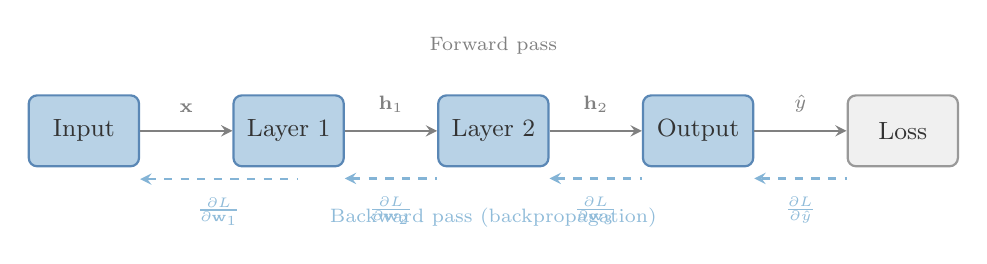
\begin{tikzpicture}[
    block/.style={draw=nodeborder, thick, fill=nodeblue,
                  rounded corners=3pt, minimum width=1.4cm,
                  minimum height=0.9cm, font=\small,
                  text=black!80},
    lossblock/.style={draw=black!40, thick, fill=black!6,
                      rounded corners=3pt, minimum width=1.4cm,
                      minimum height=0.9cm, font=\small,
                      text=black!80},
    fwd/.style={->, thick, >=stealth, black!50},
    bwd/.style={<-, thick, >=stealth, dashed, palA!55},
    lbl/.style={font=\scriptsize, text=black!50},
    bwdlbl/.style={font=\scriptsize, text=palA!50},
]

% --- Blocks ---
\node[block] (input) at (0, 0) {Input};
\node[block] (h1)    at (2.6, 0) {Layer 1};
\node[block] (h2)    at (5.2, 0) {Layer 2};
\node[block] (out)   at (7.8, 0) {Output};
\node[lossblock] (loss) at (10.4, 0) {Loss};

% --- Forward pass (solid arrows, above) ---
\draw[fwd] (input.east) -- (h1.west)
    node[midway, above=3pt, lbl] {$\mathbf{x}$};
\draw[fwd] (h1.east) -- (h2.west)
    node[midway, above=3pt, lbl] {$\mathbf{h}_1$};
\draw[fwd] (h2.east) -- (out.west)
    node[midway, above=3pt, lbl] {$\mathbf{h}_2$};
\draw[fwd] (out.east) -- (loss.west)
    node[midway, above=3pt, lbl] {$\hat{y}$};

% Forward label
\node[lbl, anchor=south] at (5.2, 0.85) {Forward pass};

% --- Backward pass (dashed arrows, below) ---
\draw[bwd] (input.south east) ++(0, -0.15)
    -- ++(2.0, 0)
    node[midway, below=3pt, bwdlbl]
    {$\frac{\partial L}{\partial \mathbf{w}_1}$};
\draw[bwd] ([yshift=-4pt]h1.south east)
    -- ([yshift=-4pt]h2.south west)
    node[midway, below=3pt, bwdlbl]
    {$\frac{\partial L}{\partial \mathbf{w}_2}$};
\draw[bwd] ([yshift=-4pt]h2.south east)
    -- ([yshift=-4pt]out.south west)
    node[midway, below=3pt, bwdlbl]
    {$\frac{\partial L}{\partial \mathbf{w}_3}$};
\draw[bwd] ([yshift=-4pt]out.south east)
    -- ([yshift=-4pt]loss.south west)
    node[midway, below=3pt, bwdlbl]
    {$\frac{\partial L}{\partial \hat{y}}$};

% Backward label
\node[bwdlbl, anchor=north] at (5.2, -0.85) {Backward pass
    (backpropagation)};

\end{tikzpicture}
\caption{Forward and backward passes through a neural network. Solid
  arrows (top): input flows left to right through each layer to
  produce a prediction and a loss. Dashed arrows (bottom): gradients
  flow right to left from the loss back through each layer, telling
  each weight how to change.}
\label{fig:forward-backward}
\end{figure}


\subsection{Network Architecture}
\label{subsec:network-architecture}

When every neuron in one layer connects to every neuron in the
next, the arrangement is called a \emph{fully connected} (or
\emph{dense}) layer. This is the most general connectivity
pattern: each output depends on every input, and each connection
has its own learned weight. Fully connected layers are the
default building block of neural networks, and they are what the
function approximator in \cref{subsec:func-approx} uses. A network
composed entirely of fully connected layers is called a \emph{multilayer
perceptron} (MLP).
\Cref{fig:mlp} illustrates a fully connected network.
Each node in the hidden layers is a neuron (\cref{fig:neuron}),
receiving all outputs from the previous layer as its inputs.

\begin{figure}[ht]
\centering
% Thesis-wide categorical color palette
% Usage: % Thesis-wide categorical color palette
% Usage: \input{figures/palette} in any figure file
%
% Muted primary colors -- print-friendly, visually distinct.
% Inspired by Cooper Union's red/blue primaries, softened for
% academic figures. Use palA-palC for data series in scatter
% plots, line charts, bar charts, etc.

\definecolor{palA}{HTML}{1F77B4}   % Tableau blue
\definecolor{palB}{HTML}{D62728}   % Tableau red
\definecolor{palC}{HTML}{2CA02C}   % Tableau green
 in any figure file
%
% Muted primary colors -- print-friendly, visually distinct.
% Inspired by Cooper Union's red/blue primaries, softened for
% academic figures. Use palA-palC for data series in scatter
% plots, line charts, bar charts, etc.

\definecolor{palA}{HTML}{1F77B4}   % Tableau blue
\definecolor{palB}{HTML}{D62728}   % Tableau red
\definecolor{palC}{HTML}{2CA02C}   % Tableau green

\definecolor{nodeblue}{HTML}{B8D2E6}
\definecolor{nodeborder}{HTML}{5A87B5}
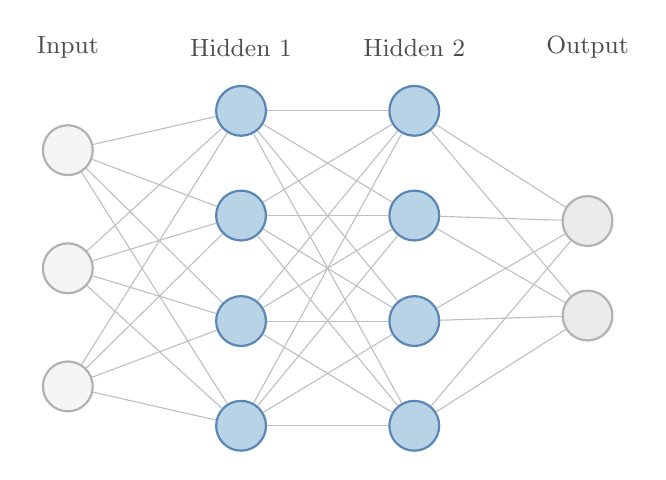
\begin{tikzpicture}[
    neuron/.style={circle, draw=nodeborder, thick, fill=nodeblue,
                   minimum size=18pt, inner sep=0pt},
    input/.style={circle, draw=black!30, thick, fill=black!4,
                  minimum size=18pt, inner sep=0pt},
    output/.style={circle, draw=black!30, thick, fill=black!8,
                   minimum size=18pt, inner sep=0pt},
    conn/.style={-, black!25},
    lbl/.style={font=\small, text=black!70},
    sublbl/.style={font=\scriptsize, text=black!50},
]

% === Main network ===

% Layer x-positions
\def\xin{0}
\def\xha{2.2}
\def\xhb{4.4}
\def\xout{6.6}

% --- Input layer (3 nodes) ---
\foreach \i/\ypos in {1/1.5, 2/0, 3/-1.5} {
    \node[input] (i\i) at (\xin, \ypos) {};
}
\node[lbl] at (\xin, 2.8) {Input};

% --- Hidden layer 1 (4 nodes) ---
\foreach \j/\ypos in {1/2.0, 2/0.67, 3/-0.67, 4/-2.0} {
    \node[neuron] (h1\j) at (\xha, \ypos) {};
}
\node[lbl] at (\xha, 2.8) {Hidden 1};

% --- Hidden layer 2 (4 nodes) ---
\foreach \k/\ypos in {1/2.0, 2/0.67, 3/-0.67, 4/-2.0} {
    \node[neuron] (h2\k) at (\xhb, \ypos) {};
}
\node[lbl] at (\xhb, 2.8) {Hidden 2};

% --- Output layer (2 nodes) ---
\foreach \l/\ypos in {1/0.6, 2/-0.6} {
    \node[output] (o\l) at (\xout, \ypos) {};
}
\node[lbl] at (\xout, 2.8) {Output};

% --- Connections ---
% Input -> Hidden 1
\foreach \i in {1,2,3} {
    \foreach \j in {1,2,3,4} {
        \draw[conn] (i\i) -- (h1\j);
    }
}
% Hidden 1 -> Hidden 2
\foreach \j in {1,2,3,4} {
    \foreach \k in {1,2,3,4} {
        \draw[conn] (h1\j) -- (h2\k);
    }
}
% Hidden 2 -> Output
\foreach \k in {1,2,3,4} {
    \foreach \l in {1,2} {
        \draw[conn] (h2\k) -- (o\l);
    }
}

\end{tikzpicture}
\vspace{6pt}
\caption{A fully connected network (multilayer perceptron) with three
  inputs, two hidden layers, and two outputs.}
\label{fig:mlp}
\end{figure}


\smallskip
A neural network maps an input to an output through a sequence of
layers. We can write this as a function $f(\mathbf{x};\,
\boldsymbol{\theta})$, where $\mathbf{x}$ is the input and
$\boldsymbol{\theta}$ is the collection of all weights and biases across
every layer. The semicolon separates the input from the parameters:
$\mathbf{x}$ changes with each example, while $\boldsymbol{\theta}$ is
fixed once training is complete.

\smallskip
Width and depth are the two axes of a network's capacity. Wider
layers compute more features at each level of abstraction; deeper
networks compose more levels. In practice, both are tuned to match
the complexity of the task.
To see how quickly parameters add up, consider a fully connected layer
with 64 neurons, each receiving 128 inputs. Each neuron has 128 weights
and one bias, so the layer has $64 \times (128 + 1) = 8{,}256$
parameters.
The number of layers, the width of each layer, and the choice of
activation function are not learned during training. These design
choices, called \emph{hyperparameters}, are fixed before training begins.

\subsection{Convolutional Layers}
\label{subsec:conv-layers}

The fully connected layers described above treat every input value
independently: each output neuron has a separate weight for every
input. For small inputs this is fine, but for images it is
impractical. An $84 \times 84 \times 4$ image has $28{,}224$
values; a single fully connected layer mapping this to 512 outputs
would require over 14 million parameters. Worse, the layer would
ignore the spatial structure of the image -- a dedicated weight
connects pixel $(3, 7)$ to each output, separate from the weight
for pixel $(3, 8)$, even though adjacent pixels contain related
information. Images are structured: nearby pixels form edges,
textures, and objects. The network should exploit this structure
rather than treat every position as independent.

\smallskip
\emph{Convolutional layers} are designed for exactly this purpose.
Instead of connecting every input to every output, a convolutional
layer applies a small matrix of weights -- a \emph{kernel} or
\emph{filter} -- that slides across the spatial extent of the
input. At each position, the kernel computes a weighted sum of the
input values it covers, producing one output value.
\Cref{fig:conv-operation} illustrates the operation: a kernel of
learned weights slides across the input, computing a weighted sum
at each position to produce one output value.

\begin{figure}[ht]
\centering
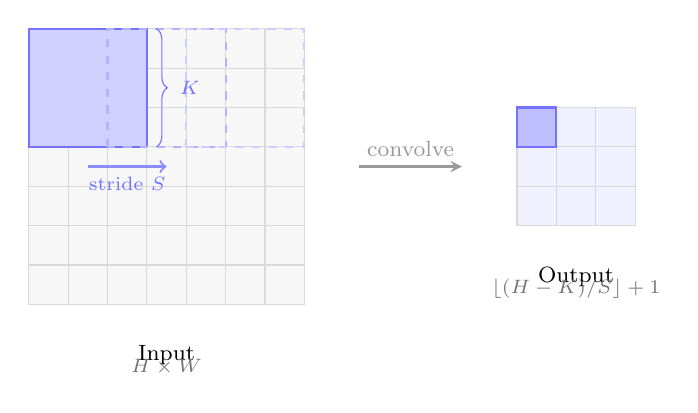
\begin{tikzpicture}[
    arr/.style={->, thick, >=stealth, black!40},
    lbl/.style={font=\footnotesize},
    sublbl/.style={font=\scriptsize, text=black!55}
]

\def\c{0.5}

% --- Input grid (7x7) ---
\foreach \x in {0,...,6} {
    \foreach \y in {0,...,6} {
        \fill[gray!6, draw=black!15]
            (\x*\c, \y*\c) rectangle ({(\x+1)*\c}, {(\y+1)*\c});
    }
}

% Kernel position 1 (solid)
\fill[blue!18, draw=blue!55, thick]
    (0, {4*\c}) rectangle ({3*\c}, {7*\c});

% Kernel position 2 (dashed, shifted by stride 2)
\draw[blue!30, thick, dashed]
    ({2*\c}, {4*\c}) rectangle ({5*\c}, {7*\c});

% Kernel position 3 (dashed, shifted again)
\draw[blue!20, thick, dashed]
    ({4*\c}, {4*\c}) rectangle ({7*\c}, {7*\c});

% Stride arrow
\draw[->, thick, blue!45]
    ({1.5*\c}, {3.5*\c}) -- ({3.5*\c}, {3.5*\c})
    node[midway, below, font=\scriptsize, blue!55] {stride $S$};

% Kernel size brace (right side of kernel)
\draw[decorate, decoration={brace, amplitude=4pt}, blue!55]
    ({3*\c + 0.12}, {7*\c}) -- ({3*\c + 0.12}, {4*\c})
    node[midway, right=5pt, font=\scriptsize, blue!55] {$K$};

% Input label
\node[lbl, anchor=north] at ({3.5*\c}, -0.4) {Input};
\node[sublbl] at ({3.5*\c}, -0.8) {$H \times W$};

% Arrow
\draw[arr] ({7*\c + 0.7}, {3.5*\c}) -- ({7*\c + 2.0}, {3.5*\c})
    node[midway, above, lbl] {convolve};

% --- Output grid (3x3) ---
\def\ox{6.2}
\foreach \x in {0,...,2} {
    \foreach \y in {0,...,2} {
        \fill[blue!6, draw=black!15]
            ({\ox + \x*\c}, {2*\c + \y*\c})
            rectangle ({\ox + (\x+1)*\c}, {2*\c + (\y+1)*\c});
    }
}

% Highlighted output cell (corresponds to kernel pos 1)
\fill[blue!25, draw=blue!55, thick]
    (\ox, {4*\c}) rectangle ({\ox + \c}, {5*\c});

% Output label
\node[lbl, anchor=north] at ({\ox + 1.5*\c}, {2*\c - 0.4}) {Output};
\node[sublbl] at ({\ox + 1.5*\c}, {2*\c - 0.8})
    {$\lfloor(H - K) / S\rfloor + 1$};

\end{tikzpicture}
\caption{Convolution operation. A $K \times K$ kernel slides across
  the input with stride $S$. Each position produces one output value.
  Dashed outlines show subsequent kernel positions.}
\label{fig:conv-operation}
\end{figure}


\smallskip
A key property of convolutions is \emph{weight sharing}: the same
kernel is applied at every spatial position, so the network detects
the same pattern regardless of where it appears in the image. A
vertical edge detector fires whether the edge is in the top-left or
the bottom-right of the frame. This is unlike a fully connected
layer, where each output has its own dedicated set of weights --
convolutions reuse the same small set of weights across the entire
input, drastically reducing the number of parameters.

\smallskip
Each convolutional layer applies many such kernels in parallel, each
learning to detect a different pattern. A layer with 32 kernels
produces 32 \emph{feature maps} -- one per kernel -- each showing
where that particular pattern was detected across the spatial extent
of the input. Successive convolutional layers build on each other:
the first might detect edges and textures, the second combines
these into shapes and parts, and the third composes parts into
higher-level structures -- the same compositional hierarchy
described for fully connected networks, but operating on spatial
features.

\smallskip
The \emph{stride} controls how many positions the kernel skips
between applications. A stride of~1 means the kernel visits every
position; a stride of~2 skips every other position, halving the
spatial dimensions. Larger strides reduce the output size more
aggressively, trading spatial resolution for computational
efficiency. \Cref{fig:stride-effect} illustrates the trade-off: a
larger stride means the kernel visits fewer positions and the output
shrinks accordingly.

\begin{figure}[ht]
\centering
% Thesis-wide categorical color palette
% Usage: % Thesis-wide categorical color palette
% Usage: \input{figures/palette} in any figure file
%
% Muted primary colors -- print-friendly, visually distinct.
% Inspired by Cooper Union's red/blue primaries, softened for
% academic figures. Use palA-palC for data series in scatter
% plots, line charts, bar charts, etc.

\definecolor{palA}{HTML}{1F77B4}   % Tableau blue
\definecolor{palB}{HTML}{D62728}   % Tableau red
\definecolor{palC}{HTML}{2CA02C}   % Tableau green
 in any figure file
%
% Muted primary colors -- print-friendly, visually distinct.
% Inspired by Cooper Union's red/blue primaries, softened for
% academic figures. Use palA-palC for data series in scatter
% plots, line charts, bar charts, etc.

\definecolor{palA}{HTML}{1F77B4}   % Tableau blue
\definecolor{palB}{HTML}{D62728}   % Tableau red
\definecolor{palC}{HTML}{2CA02C}   % Tableau green


%% Panel (a): Stride 1
\begin{subfigure}[t]{0.45\textwidth}
\centering
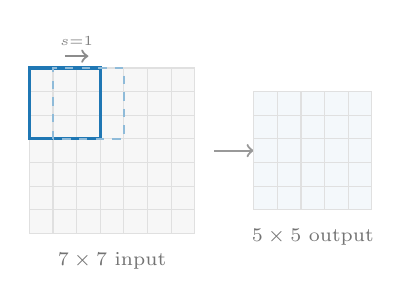
\begin{tikzpicture}[
    lbl/.style={font=\scriptsize, text=black!55},
]
\def\c{0.3}

% 7x7 input grid (empty)
\foreach \x in {0,...,6} {
    \foreach \y in {0,...,6} {
        \fill[gray!6, draw=black!12]
            (\x*\c, \y*\c) rectangle ++(\c, \c);
    }
}

% Kernel position 1 (solid blue, cols 0-2)
\draw[palA, very thick]
    (0, {4*\c}) rectangle ({3*\c}, {7*\c});

% Kernel position 2 (dashed, cols 1-3 -- one cell shift)
\draw[palA!50, thick, dashed]
    ({1*\c}, {4*\c}) rectangle ({4*\c}, {7*\c});

% Stride arrow above grid
\draw[->, thick, black!45]
    ({1.5*\c}, {7*\c + 0.15}) -- ({2.5*\c}, {7*\c + 0.15})
    node[midway, above, font=\tiny, text=black!50] {$s{=}1$};

% Input label
\node[lbl, anchor=north] at ({3.5*\c}, -0.12) {$7 \times 7$ input};

% Arrow to output
\draw[->, thick, black!40]
    ({7*\c + 0.25}, {3.5*\c}) -- ++(0.5, 0);

% 5x5 output grid
\def\ox{2.85}
\def\oy{0.3}
\foreach \x in {0,...,4} {
    \foreach \y in {0,...,4} {
        \fill[palA!5, draw=black!12]
            ({\ox + \x*\c}, {\oy + \y*\c})
            rectangle ++({\c}, {\c});
    }
}
\node[lbl, anchor=north] at ({\ox + 2.5*\c}, {\oy - 0.12})
    {$5 \times 5$ output};

\end{tikzpicture}
\subcaption{Stride $1$: the kernel shifts one cell per step.}
\label{fig:stride-one}
\end{subfigure}
\hfill
%% Panel (b): Stride 2
\begin{subfigure}[t]{0.45\textwidth}
\centering
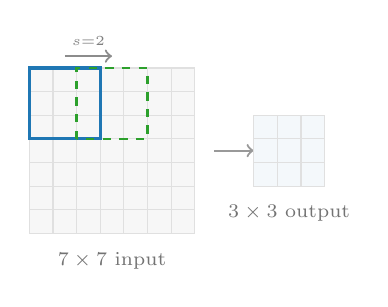
\begin{tikzpicture}[
    lbl/.style={font=\scriptsize, text=black!55},
]
\def\c{0.3}

% 7x7 input grid (empty)
\foreach \x in {0,...,6} {
    \foreach \y in {0,...,6} {
        \fill[gray!6, draw=black!12]
            (\x*\c, \y*\c) rectangle ++(\c, \c);
    }
}

% Kernel position 1 (solid blue, cols 0-2)
\draw[palA, very thick]
    (0, {4*\c}) rectangle ({3*\c}, {7*\c});

% Kernel position 2 (dashed green, cols 2-4 -- two cell shift)
\draw[palC, thick, dashed]
    ({2*\c}, {4*\c}) rectangle ({5*\c}, {7*\c});

% Stride arrow above grid
\draw[->, thick, black!45]
    ({1.5*\c}, {7*\c + 0.15}) -- ({3.5*\c}, {7*\c + 0.15})
    node[midway, above, font=\tiny, text=black!50] {$s{=}2$};

% Input label
\node[lbl, anchor=north] at ({3.5*\c}, -0.12) {$7 \times 7$ input};

% Arrow to output
\draw[->, thick, black!40]
    ({7*\c + 0.25}, {3.5*\c}) -- ++(0.5, 0);

% 3x3 output grid (smaller than panel a)
\def\ox{2.85}
\def\oy{0.6}
\foreach \x in {0,...,2} {
    \foreach \y in {0,...,2} {
        \fill[palA!5, draw=black!12]
            ({\ox + \x*\c}, {\oy + \y*\c})
            rectangle ++({\c}, {\c});
    }
}
\node[lbl, anchor=north] at ({\ox + 1.5*\c}, {\oy - 0.12})
    {$3 \times 3$ output};

\end{tikzpicture}
\subcaption{Stride $2$: the kernel shifts two cells per step.}
\label{fig:stride-two}
\end{subfigure}

\caption{Effect of stride on output size. Both panels use the same
  $7 \times 7$ input and $3 \times 3$ kernel. A larger stride means
  fewer kernel positions and a smaller output feature map.}
\label{fig:stride-effect}
\end{figure}


\smallskip
In a typical architecture, several convolutional layers are
followed by one or more fully connected layers. The convolutional
layers progressively extract spatial features while reducing the
spatial dimensions; the fully connected layers then read from the
resulting feature maps to produce the final output. This
combination -- convolutional layers for spatial processing, fully
connected layers for the final mapping -- is the foundation of most
image-processing neural networks, including the one used in the
deep Q-network described in \cref{sec:dqn}.

\subsection{Representations}
\label{subsec:representations}

A neural network does not just map input to output. Each
intermediate layer computes a transformation of the input, and
these intermediate activations -- the values produced by the
neurons in a given layer -- are themselves a description of the
input. A different description from the raw pixels, expressed in
a new coordinate system that (ideally) makes the task easier. These
intermediate activations are the network's \emph{representation}
of the input.

\smallskip
In many architectures, the early layers progressively compress the
input into a lower-dimensional intermediate form, and the later
layers read from this compressed form to produce the output. The
early layers are the \emph{encoder}; the later layers are the
\emph{task head}. The compressed intermediate form is the
\emph{representation} or \emph{latent vector}, and the space of
all possible such vectors is the \emph{latent space}.

\smallskip
To make this concrete: an $84 \times 84 \times 4$ image has
$28{,}224$ pixel values. After passing through an encoder -- several
layers that progressively reduce the spatial dimensions -- the
result might be a vector of 512 values. Those 512 numbers are the
representation: a summary of whatever the encoder has learned to
extract from the image. The full input lives in a $28{,}224$-dimensional
space; the representation lives in a $512$-dimensional space. Every
input maps to one point in this latent space, and -- if the encoder
has learned well -- inputs that are similar in task-relevant ways
map to nearby points. \Cref{fig:encoder-latent-space} illustrates
this decomposition: the encoder narrows the input into a compact
representation, and the task head reads from it to produce the
output.

\begin{figure}[ht]
\centering
% Thesis-wide categorical color palette
% Usage: % Thesis-wide categorical color palette
% Usage: \input{figures/palette} in any figure file
%
% Muted primary colors -- print-friendly, visually distinct.
% Inspired by Cooper Union's red/blue primaries, softened for
% academic figures. Use palA-palC for data series in scatter
% plots, line charts, bar charts, etc.

\definecolor{palA}{HTML}{1F77B4}   % Tableau blue
\definecolor{palB}{HTML}{D62728}   % Tableau red
\definecolor{palC}{HTML}{2CA02C}   % Tableau green
 in any figure file
%
% Muted primary colors -- print-friendly, visually distinct.
% Inspired by Cooper Union's red/blue primaries, softened for
% academic figures. Use palA-palC for data series in scatter
% plots, line charts, bar charts, etc.

\definecolor{palA}{HTML}{1F77B4}   % Tableau blue
\definecolor{palB}{HTML}{D62728}   % Tableau red
\definecolor{palC}{HTML}{2CA02C}   % Tableau green

\definecolor{encfade}{HTML}{B8D2E6}
\definecolor{reprfill}{HTML}{D6E8F4}
\definecolor{headfill}{HTML}{E8E8E8}
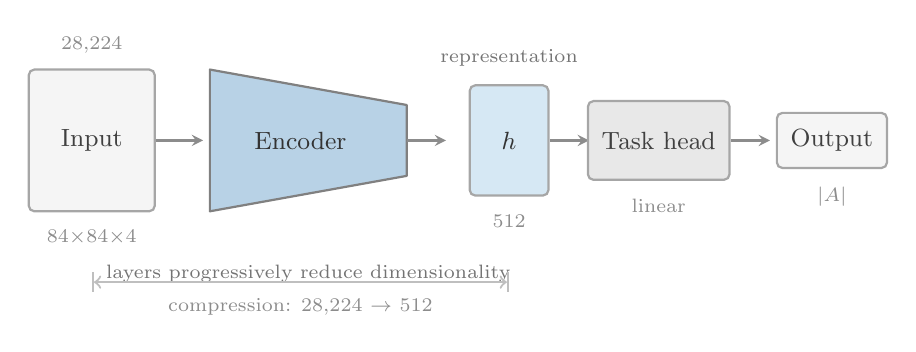
\begin{tikzpicture}[
    arr/.style={->, thick, >=stealth, black!45},
    lbl/.style={font=\small, text=black!80},
    dimlbl/.style={font=\scriptsize, text=black!45},
    sublbl/.style={font=\scriptsize, text=black!55},
    block/.style={draw=black!35, thick, rounded corners=2pt,
                  minimum height=0.8cm, font=\small,
                  text=black!75, inner sep=5pt},
]

% --- Input ---
\node[block, fill=black!4, minimum width=1.6cm,
      minimum height=1.8cm] (input) at (0, 0) {Input};
\node[dimlbl, below=3pt] at (input.south) {$84{\times}84{\times}4$};
\node[dimlbl, above=2pt] at (input.north) {28{,}224};

\draw[arr] (input.east) -- ++(0.6, 0);

% --- Encoder (trapezoid matching single-objective.tex) ---
\fill[encfade, draw=black!50, thick, line join=round]
    (1.5, -0.9) -- (1.5, 0.9) -- (4.0, 0.45) -- (4.0, -0.45)
    -- cycle;
\node[lbl] at (2.65, 0) {Encoder};
\node[sublbl, below=16pt] at (2.75, -0.9) {layers progressively
    reduce dimensionality};

\draw[arr] (4.0, 0) -- ++(0.5, 0);

% --- Representation (bottleneck) ---
\node[block, fill=reprfill, minimum width=1.0cm,
      minimum height=1.4cm, text=black!80,
      font=\small\bfseries] (repr) at (5.3, 0) {$h$};
\node[dimlbl, below=3pt] at (repr.south) {512};
\node[sublbl, above=3pt] at (repr.north) {representation};

\draw[arr] (repr.east) -- ++(0.5, 0);

% --- Task head ---
\node[block, fill=headfill, minimum width=1.2cm,
      minimum height=1.0cm] (head) at (7.2, 0) {Task head};
\node[dimlbl, below=3pt] at (head.south) {linear};

\draw[arr] (head.east) -- ++(0.5, 0);

% --- Output ---
\node[block, fill=black!4, minimum width=1.0cm,
      minimum height=0.7cm] (output) at (9.4, 0) {Output};
\node[dimlbl, below=3pt] at (output.south) {$|A|$};

% --- Dimensionality annotation (spanning arrow) ---
\draw[black!25, thick, |<->|]
    (0, -1.8) -- (5.3, -1.8)
    node[midway, below=2pt, dimlbl] {compression:
    28{,}224 $\to$ 512};

\end{tikzpicture}
\caption{Encoder, representation, and task head. The encoder
  compresses a high-dimensional input into a low-dimensional
  representation~$h$. The task head reads from this representation
  to produce the output. The same pattern appears in DQN
  (\cref{sec:dqn}), where the encoder is a convolutional network
  and the task head maps representations to Q-values.}
\label{fig:encoder-latent-space}
\end{figure}


\smallskip
What makes a representation good? A good representation captures
the structure that matters for the task and discards what does not.
Consider a network trained to classify handwritten digits. The raw
input is a grid of pixel intensities, but the classification
depends on stroke topology -- the spatial arrangement of lines and
curves -- not on ink thickness, pen angle, or exact pixel positions.
If the encoder's 512-dimensional representation separates the ten
digit classes into distinct clusters in latent space, then the task
head -- even a single linear layer -- can easily draw boundaries
between them. If the representation is a jumble where different
digits overlap, no task head can reliably classify them.

\smallskip
This is why representations matter so much: they determine what
information is available to the task head. A powerful task head
cannot compensate for a poor representation, because the
information was lost during encoding. Conversely, a good
representation makes the task head's job easy, even if the task
head is simple. This principle motivates \emph{linear probing} --
attaching a single linear layer to a frozen representation and
measuring what it can predict. High accuracy means the information
is linearly accessible in the representation; low accuracy means it
is either absent or encoded in a way that requires nonlinear
decoding.

\smallskip
When comparing two representations -- for instance, checking
whether a predicted future representation matches an actual future
representation -- we often care about direction rather than
magnitude. Two vectors might differ in length but point in the same
direction, indicating they encode the same information at different
scales. \emph{Cosine similarity} measures this:
%
\begin{equation}
\label{eq:cosine-similarity}
\text{cos}(\mathbf{a}, \mathbf{b})
  = \frac{\mathbf{a} \cdot \mathbf{b}}
         {\|\mathbf{a}\|\;\|\mathbf{b}\|}.
\end{equation}
%
A cosine similarity of $1$ means the two vectors point in the same
direction (identical encoding); $0$ means they are orthogonal
(completely unrelated); $-1$ means they point in opposite
directions. For example, two 512-dimensional representations with
cosine similarity $0.95$ encode nearly the same information, while
a pair with similarity $0.1$ share almost nothing. Cosine
similarity appears throughout this work: it is the loss function
for SPR (\cref{subsec:spr}), the metric for transition model
analysis, and a tool for comparing representations across
experimental conditions.

\smallskip
In the DQN architecture described in the next section, the
convolutional layers are the encoder and the 512-dimensional
activation of the fully connected layer is the representation.
The Q-values are computed from this representation by the task head
-- a single linear output layer. Whether the Q-learning loss alone
shapes this representation well enough for the agent to learn
effectively, or whether additional training signals can improve it,
is the central question of this thesis.
